\documentclass[aspectratio=169]{beamer}
\usetheme{simple}
\usepackage[english]{babel}
\usepackage[utf8]{inputenc} 
\usepackage{lmodern}
\usepackage{ragged2e}
\usefonttheme[onlymath]{serif} 
\usepackage[scale=2]{ccicons} 
% \setbeamertemplate{caption}[numbered]
\usepackage{copyrightbox}
\DeclareMathOperator*{\argmin}{arg\,min}

\usepackage{graphicx,hyperref,url,pgfplots}
\usepackage{amsmath} 
\usepackage{array,booktabs}
\pgfplotsset{compat=1.13}
\usepackage{bibentry}
\usepackage[alf,abnt-etal-list=0,abnt-etal-cite=2]{abntex2cite}
\usepackage[normalem]{ulem}
\PassOptionsToPackage{demo}{graphicx}
\def\HiLi{\leavevmode\rlap{\hbox to \hsize{\color{yellow!50}\leaders\hrule height .8\baselineskip depth .5ex\hfill}}}

\usepackage[
    type={CC},
    modifier={by-nc-sa},
    version={4.0},
]{doclicense}

\setbeamercovered{invisible} 
\newcommand{\df}[1]{\,\mathrm{d}#1}
\newcommand{\parcial}[3]{\dfrac{\partial^{#1}#2}{\partial #3^{#1}}}
\newcommand{\cpright}[2]{\copyrightbox[b]{#1}{\tiny Source: #2}}
%Tikz
\newcommand{\tikzRot}{0}
\newcommand{\tikzTrans}{(0,0)}
\newcommand{\tikzShowrobot}{0}
\newcommand{\tikzOneCenter}{0}



\usepackage{tikz}
\usetikzlibrary{automata,positioning}
\usepackage{xcolor}
\usetikzlibrary{scopes}
\usepackage{verbatim}
\usetikzlibrary{patterns}
\usepackage{algorithm}
\usepackage{algpseudocode}
\def\NoNumber#1{{\def\alglinenumber##1{}\State #1}\addtocounter{ALG@line}{-1}}

\usepackage{listings}
  \lstdefinestyle{ascii-tree}{
    literate={├}{|}1 {─}{--}1 {└}{+}1 
  }
	\definecolor{codegreen}{rgb}{0,0.6,0}
	\definecolor{codegray}{rgb}{0.5,0.5,0.5}
	\definecolor{codepurple}{rgb}{0.58,0,0.82}
	\definecolor{backcolour}{rgb}{0.92,0.92,0.92}
	\lstset{language=Python, 
	backgroundcolor=\color{backcolour},   
	commentstyle=\color{codegreen},
	keywordstyle=\color{magenta},
	numberstyle=\tiny\color{codegray},
	stringstyle=\color{codepurple},
	basicstyle=\fontsize{8}{11}\ttfamily,
	frame=lines,
%	numbers=left,
	tabsize=2,
	morekeywords={models, lambda, forms},
	showstringspaces=false}

\usepackage{catchfile}
\newcommand{\getenv}[2][]{%
	\CatchFileEdef{\temp}{"|kpsewhich --var-value #2"}{\endlinechar=-1}%
	\if\relax\detokenize{#1}\relax\temp\else\let#1\temp\fi}

\getenv[\BIBREF]{RM_REFERENCES}


% --------------------------------------------------------------------------------------------

\title{Mobile Robots}
\subtitle{Pose Estimation - ICP Algorithm}
\date{\today}
\author[Jeferson José de Lima]{
  \textbf{Professor}: Jeferson José de Lima}
\institute{Academic Department of Informatics (DAINF) \\ Federal University of Technology - Paraná (UTFPR) at Pato Branco, PR, Brazil}

\begin{document}
\maketitle
\justify

\begin{frame}{Useful Information}

	\begin{block}{License}
        \doclicenseThis
    \end{block}

	\begin{block}{links:}
		\begin{enumerate}
			\item \href{https://gitlab.com/cursoseaulas/robotica-movel/-/wikis/home}{Mobile Robots - Gitlab Page}
			\item \BIBREF
		\end{enumerate}
	\end{block}
\end{frame}

\begin{frame}{Pose Estimation}
	\framesubtitle{}
	After this lesson, you will able to:
	\begin{itemize}
		\item Describe the point LiDAR points and how it can be used for state estimation
		\item Implement the Iterative Closest Point (ICP) algorithm. 
	\end{itemize}
\end{frame}

 
\begin{frame}{Pose Estimation}
	\framesubtitle{Point Clouds}

	\textcolor{purple}{\textbf{Point Cloud}} 

	\begin{itemize}
		\item A point cloud is a set of data points in space. The points represent a 3D shape or object. Each point has its set of $X$, $Y$ and $Z$ coordinates.\footnote[frame]{\textcolor{blue}{\textbf{More info}}: \href{https://www.zivid.com/3d-point-cloud-examples/}{3D Cloud Point Examples}}
	\end{itemize}

	\addtolength{\jot}{5em}
	\begin{align*}
		\cpright{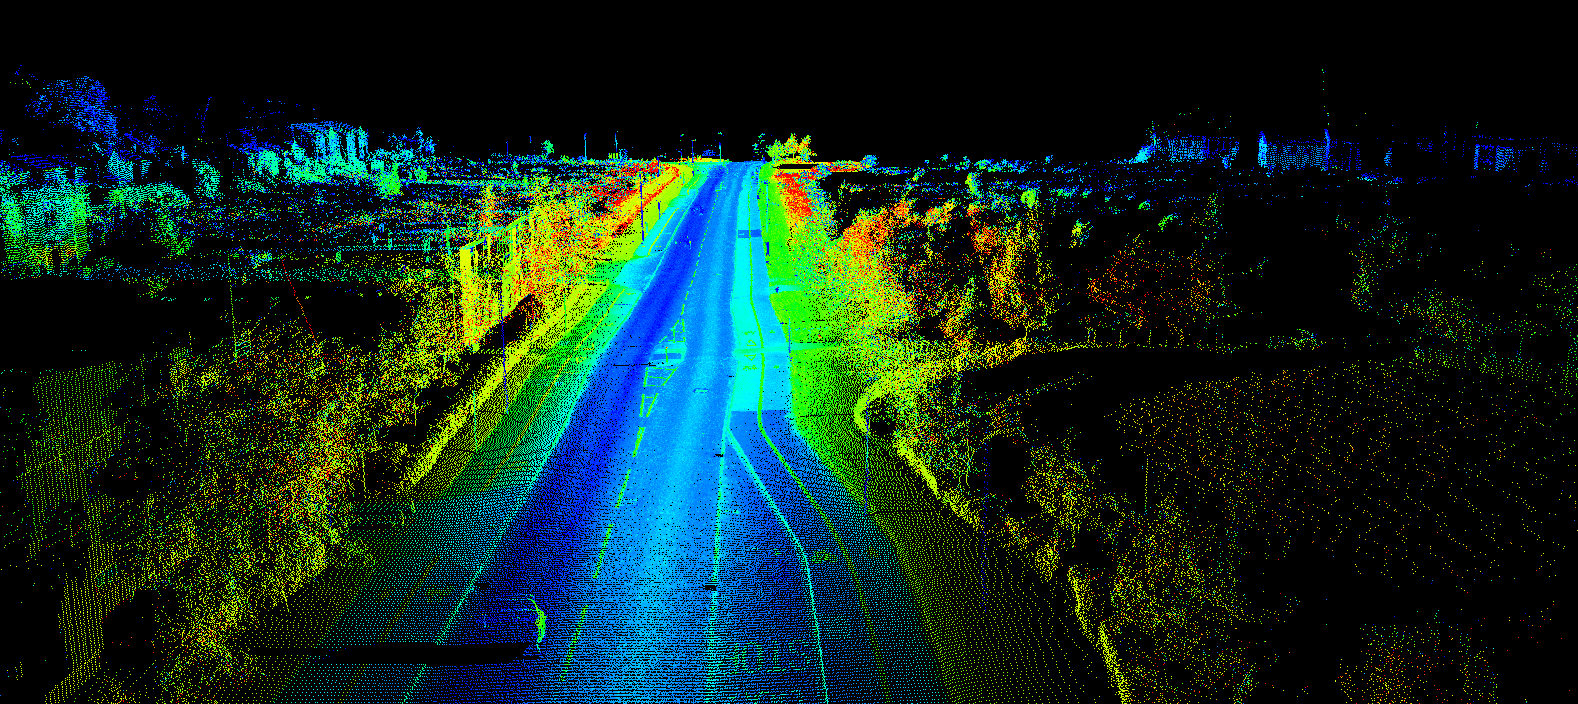
\includegraphics[width=0.45\textwidth]{./images/pcexample1.png}}
		{https://www.zivid.com/3d-point-cloud-examples/} & &
		\cpright{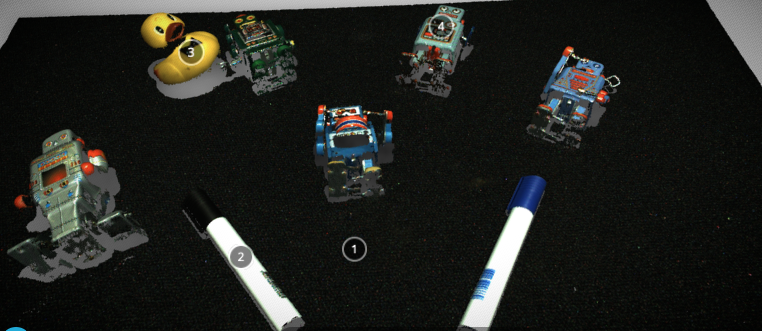
\includegraphics[width=0.45\textwidth]{./images/pcexample2.png}}
		{https://www.geospatialworld.net/news/} 
	\end{align*}
		

\end{frame}


\begin{frame}{Pose Estimation}
	\framesubtitle{\textcolor{purple}{What motion of the car best aligns the two point clouds?}}
		
    \begin{columns}
        \begin{column}[c]{0.5\textwidth}
            \def\iangle{35} % Angle of the inclined plane
\def\down{0}
\def\arcr{0.7cm} % Radius of the arc used to indicate angles
\newcommand\centerofmass{%
    \tikz[radius=0.2em, red] {%
        \fill (0,0) -- ++(0.2em,0) arc [start angle=0,end angle=90] -- ++(0,-0.4em) arc [start angle=270, end angle=180];%
        \draw (0,0) circle;%
    }%
}

\begin{tikzpicture}[
    force/.style={>=latex,draw=blue,fill=blue},
    axis/.style={densely dashed,gray,font=\small},
    M/.style={rectangle,draw,fill=lightgray,minimum size=0.7cm,thin},
    m/.style={rectangle,draw=black,fill=lightgray,minimum size=0.3cm,thin},
    plane/.style={draw=black,fill=blue!10},
    string/.style={draw=red, thick},
    pulley/.style={thick},
    wheel/.style={fill=black, rounded corners=1.5pt},
]

    \begin{scope}
        \node[draw,anchor=south west,pattern=north west lines,minimum width=2cm,minimum height=1cm] (Ob1) at (0,2) {};
        \node[draw,anchor=south west,pattern=north west lines,minimum width=1cm,minimum height=1cm] (Ob2) at (2.5,-1.5) {};
    \end{scope}

     \begin{scope}[rotate=0]
        \node[M,transform shape] (M1) at (-2,-1) {\centerofmass};
        % Draw axes and help lines
        % {[axis,->]
        %     \draw (M1) -- ++(0,2) node(y1_axis)[right] {$y'$};
        % }
        % Forces
        {[force,->]
            % Assuming that Mg = 1. The normal force will therefore be cos(alpha)
            \draw (M1.east) -- ++(1,0) node[above, blue] {};
        }
        \draw[wheel, fill=gray] (M1.south west) rectangle ++(.4,-.1) node[]{};
        \draw[wheel, fill=gray] (M1.north west) rectangle ++(.4,.1)  node[]{};

        \node[] at (-2,-2) {$\textcolor{red}{\mathbf{P}_{t}}$};
    \end{scope}

    \onslide<1->


    \draw[, ->] (-2,-1) -- ++(2,0) node[below] {$x$};
    \draw[, ->] (-2,-1) -- ++(0,2) node(y_axis)[right] {$y$};
    \draw[gray, ->] (-2,-1) -- ++(-.5,-.5) node[left] {$z$};

    \onslide<2>

        % lidar
        \draw[axis, gray] (M1.center) -- (Ob1.west) node[] {x};
        \draw[axis, gray] (M1.center) -- (Ob1.south west) node[] {x};
        \draw[axis, gray] (M1.center) -- (Ob1.south) node[] {x};
        \draw[axis, gray] (M1.center) -- (Ob1.south east) node[] {x};
        %%
        \draw[axis, gray] (M1.center) -- (Ob2.north west) node[] {x};
        \draw[axis, gray] (M1.center) -- (Ob2.west) node[] {x};
        \draw[axis, gray] (M1.center) -- (Ob2.south west) node[] {x};
        \draw[axis, gray] (M1.center) -- (Ob2.north east) node[] {x};

    \onslide<3->
    %% Free body diagram of M
    \begin{scope}[rotate=\iangle]
        \node[M,transform shape] (M2) at (1,-0.5) {\centerofmass};
        % Draw axes and help lines
        {[axis,->]
            % \draw (M2) -- ++(0,2) node(y1_axis)[right] {};
            % \draw (M2) -- ++(2,0) node[right] {};
            % Indicate angle. The code is a bit awkward.
            \draw[solid,shorten >=0.5pt, xshift=30, yshift=-15] (\down-\iangle:\arcr)
                arc(\down-\iangle:\down:\arcr);
            \node[xshift=35, yshift=2] at (\down-0.5*\iangle:1.3*\arcr) {$\phi$};
        }
        % Forces
        {[force,->]
            % Assuming that Mg = 1. The normal force will therefore be cos(alpha)
            \draw (M2.east) -- ++(1,0) node[above, blue] {};
        }
        \draw[wheel] (M2.south west) rectangle ++(.4,-.1) node[below]{};
        \draw[wheel] (M2.north west) rectangle ++(.4,.1)  node[left]{};
        \node[] at (0.5,0.5) {$\textcolor{blue}{\mathbf{P}_{t+1}}$};
    \end{scope}
    % Draw gravity force. The code is put outside the rotated
    % scope for simplicity. No need to do any angle calculations. 
    \draw[axis,] (M2.center) -- ++(1,0) node[below] {};

    \onslide<4>

    % lidar
    \draw[red] (M2.center) -- (Ob1.south west) node[] {x};
    \draw[red] (M2.center) -- (Ob1.south) node[] {x};
    \draw[red] (M2.center) -- (Ob1.south east) node[] {x};
    %%
    \draw[red] (M2.center) -- (Ob2.north west) node[] {x};
    \draw[red] (M2.center) -- (Ob2.west) node[] {x};
    \draw[red] (M2.center) -- (Ob2.south west) node[] {x};
    \draw[red] (M2.center) -- (Ob2.north east) node[] {x};



    % \node[right, gray,font=\small, xshift=8] at (M1.center) {$\{B\}$};
    % %%
    % \node[left, gray,font=\small, xshift=-10] at (0,0) {$\{A\}$};
\end{tikzpicture}

        \end{column}
        \begin{column}[c]{0.5\textwidth}
			\vspace{0.4in}
            \def\iangle{35} % Angle of the inclined plane
\def\down{0}
\def\arcr{0.7cm} % Radius of the arc used to indicate angles
\newcommand\centerofmass{%
    \tikz[radius=0.2em, red] {%
        \fill (0,0) -- ++(0.2em,0) arc [start angle=0,end angle=90] -- ++(0,-0.4em) arc [start angle=270, end angle=180];%
        \draw (0,0) circle;%
    }%
}

\begin{tikzpicture}[
    force/.style={>=latex,draw=blue,fill=blue},
    axis/.style={densely dashed,gray,font=\small},
    M/.style={rectangle,draw,fill=lightgray,minimum size=0.7cm,thin},
    m/.style={rectangle,draw=black,fill=lightgray,minimum size=0.3cm,thin},
    plane/.style={draw=black,fill=blue!10},
    string/.style={draw=red, thick},
    pulley/.style={thick},
    wheel/.style={fill=black, rounded corners=1.5pt},
]

    %% Free body diagram of M
    \begin{scope}[rotate=\iangle]
        \node[] (M)  at (1,-0.5){\centerofmass};
        % \node[below, purple] at (M) {${}^B_A\mathbf{P}$};
        % Draw axes and help lines
        {[axis,->]
            \draw (M.center) -- ++(0,2) node(y1_axis)[right] {$y_M$};
            \draw (M.center) -- ++(2,0) node[right] {$x_M$};
            % Indicate angle. The code is a bit awkward.
            \draw[solid,shorten >=0.5pt, xshift=30, yshift=-15] (\down-\iangle:\arcr) arc(\down-\iangle:\down:\arcr);
            \node[xshift=45, yshift=2, brown]at (\down-0.5*\iangle:1.3*\arcr) {$\mathbf{R}_z(\theta)$};
        }
        % Forces
        {[force,->]
            % Assuming that Mg = 1. The normal force will therefore be cos(alpha)
            \draw (M.center) -- ++(1,0) node[above, blue] {$v_M$};
        }
    \end{scope}
    % Draw gravity force. The code is put outside the rotated
    % scope for simplicity. No need to do any angle calculations. 
    \draw[axis,] (M.center) -- ++(1,0) node[below] {};
    %%
    \node[right, gray,font=\small, xshift=8] at (y1_axis) {$\{M\}$};
    %%
    \draw[, ->] (-2,-1) -- ++(2,0) node[below] {$x$};
    \draw[, ->] (-2,-1) -- ++(0,2) node(y_axis)[right] {$y$};
    \draw[gray, ->] (-2,-1) -- ++(-.5,-.5) node[left] {$z$};
    % \node[left, gray,font=\small, xshift=-10] at (y_axis) {$\{I\}$};
    \draw [densely dashed,purple] (-2,-1)-- (M.center) node[above, midway] {$\mathbf{Q}$};
\end{tikzpicture}

  
        \end{column}
    \end{columns}

	\vspace{0.1in}

	\begin{block}{\textcolor{blue}{We just need to solve for the transformation $\textcolor{gray}{\mathbf{T}(\textcolor{brown}{\theta}, \textcolor{purple}{\mathbf{Q}})}$:}}

	\begin{equation*}
        \begin{bmatrix}
            \color{blue}{ \mathbf{P}_{t+1}} \\ 1
        \end{bmatrix}
        =
        \left[
            \begin{matrix}
                  & \color{brown}{\mathbf{R}_z(\theta)} &   \\ \hline
                0 & 0 & 0 \\
            \end{matrix} \right.
            \left.
            \vline
            \begin{matrix}
                \color{purple}{\mathbf{Q}} \\ \hline
                1
            \end{matrix} \right]
        \begin{bmatrix}
            \color{red}{\mathbf{P}_{t}} \\
            1
        \end{bmatrix}
		\text{, or }
		\begin{bmatrix}
            \color{blue}{ \mathbf{P}_{t+1}} \\ 1
        \end{bmatrix}
        =
        \mathbf{T}(\textcolor{brown}{\theta}, \textcolor{purple}{\mathbf{Q}})
        \begin{bmatrix}
            \color{red}{\mathbf{P}_{t}} \\
            1
        \end{bmatrix}
    \end{equation*}
\end{block}
\end{frame}

\begin{frame}{Pose Estimation}
	\framesubtitle{2D LiDAR Data Example}

	\textbf{Turtlebot3 and 2D LiDAR Data}:

	\begin{figure}
		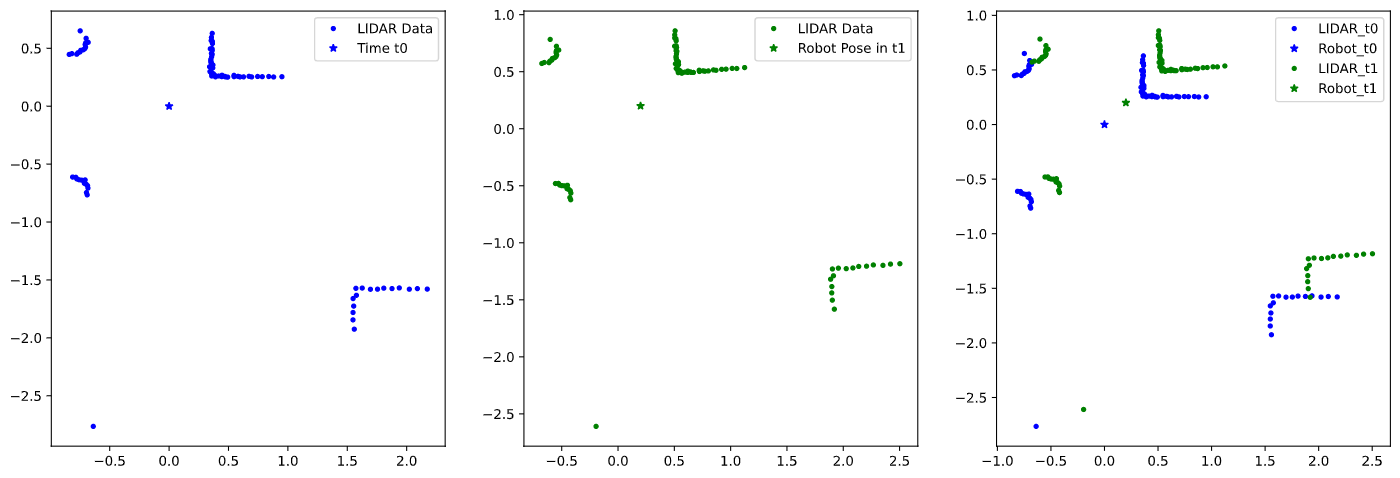
\includegraphics[width=1\textwidth]{./images/lidarExample.png}
	\end{figure}
\end{frame}


\begin{frame}{Pose Estimation}
	\framesubtitle{2D LiDAR Data Example}

	\textbf{Velodyne 3D LiDAR Sensor}:

	\begin{figure}
		\cpright{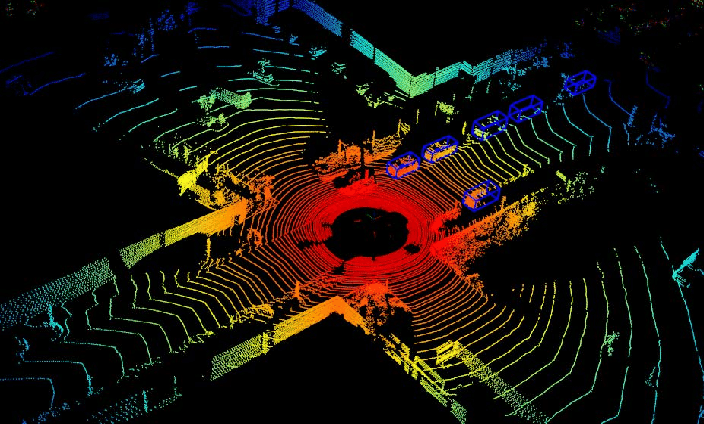
\includegraphics[width=0.6\textwidth]{./images/velodyne_sensor.png}}
		{\cite{wang2015fast}}
		\caption{Point cloud of the Velodyne LiDAR.}
	\end{figure}
\end{frame} 
 
% \begin{frame}[fragile, t]{Pose Estimation}
% 	\framesubtitle{The Iterative Closest Point (ICP) Algorithm}
% 	\begin{minipage}{0.6\textwidth}

% 	\begin{block}{}
% 		\textcolor{red}{\textbf{Problem}: We don’t know which points correspond to each other}
% 	\end{block}

% 	\vspace{0.3in}

% 	\textcolor{purple}{\textbf{The Iterative Closest Point (ICP) Algorithm}}

%     \begin{itemize}
%         \item \textbf{Intuition}: When the optimal motion is found, corresponding points will be closer to each other than to other points
%         \item  \textbf{Heuristic}: For each point, the best candidate for a corresponding point is the point that is closest to it right now
%     \end{itemize}

% \end{minipage}
% \begin{minipage}{0.4\textwidth}
% 	\begin{figure}
% 		\renewcommand{\tikzRot}{40}
% 		\renewcommand{\tikzTrans}{(6,0)}
% 		\renewcommand{\tikzShowrobot}{1}
% 		\resizebox{0.8\textwidth}{!}{
% 		\begin{tikzpicture}
	\begin{scope}
		\node [fill=blue, draw=black, shape=circle] (0) at (-2, 6) {};
		\node [fill=blue, draw=black, shape=circle] (1) at (-2, 4.75) {};
		\node [fill=blue, draw=black, shape=circle] (2) at (-1.5, 4.5) {};
		\node [fill=blue, draw=black, shape=circle] (3) at (-0.75, 4.5) {};
		\node [fill=blue, draw=black, shape=circle] (4) at (0.5, 4.5) {};
		\node [fill=blue, draw=black, shape=circle] (5) at (1.5, 4.5) {};
		\node [fill=blue, draw=black, shape=circle] (6) at (2.5, 4.5) {};

		\node [fill=blue, draw=black, shape=circle] (7) at (5.5, -0.5) {};
		\node [fill=blue, draw=black, shape=circle] (8) at (5.5, -1.5) {};
		\node [fill=blue, draw=black, shape=circle] (9) at (5.5, -2.75) {};
		\node [fill=blue, draw=black, shape=circle] (10) at (5.25, -3.5) {};
		\node [fill=blue, draw=black, shape=circle] (11) at (4, -3.75) {};
		\node [fill=blue, draw=black, shape=circle] (12) at (2.75, -4) {};
		\node [fill=blue, draw=black, shape=circle] (13) at (2.25, -4.5) {};
		\node [fill=blue, draw=black, shape=circle] (14) at (2.25, -5.5) {};
		\ifnum\tikzShowrobot=1
			\node [fill=gray, draw=black, shape=circle] (Robot) at (-4, 0.25) {\textcolor{white}{\huge Robot}};
		\fi
		\node[above, xshift=45, yshift=13] at (0) {\Huge{$\textcolor{blue}{\mathbf{P}_{t+1}}$}};
		\ifnum\tikzOneCenter=0
			\node [fill=gray, shape=circle] (c1) at (2, 0) {};
			\node [below, yshift = -8] at (c1) {\Huge{$\mathbf{c}^{t+1}$}};
		\fi
	\end{scope}
	\begin{scope}[rotate=\tikzRot, shift={\tikzTrans}]
		\node [fill=red, draw=black, shape=circle] (b0) at (-2, 6) {};
		\node [fill=red, draw=black, shape=circle] (b1) at (-2, 4.75) {};
		\node [fill=red, draw=black, shape=circle] (b2) at (-1.5, 4.5) {};
		\node [fill=red, draw=black, shape=circle] (b3) at (-0.75, 4.5) {};
		\node [fill=red, draw=black, shape=circle] (b4) at (0.5, 4.5) {};
		\node [fill=red, draw=black, shape=circle] (b5) at (1.5, 4.5) {};
		\node [fill=red, draw=black, shape=circle] (b6) at (2.5, 4.5) {};

		\node [fill=red, draw=black, shape=circle] (b7) at (5.5, -0.5) {};
		\node [fill=red, draw=black, shape=circle] (b8) at (5.5, -1.5) {};
		\node [fill=red, draw=black, shape=circle] (b9) at (5.5, -2.75) {};
		\node [fill=red, draw=black, shape=circle] (b10) at (5.25, -3.5) {};
		\node [fill=red, draw=black, shape=circle] (b11) at (4, -3.75) {};
		\node [fill=red, draw=black, shape=circle] (b12) at (2.75, -4) {};
		\node [fill=red, draw=black, shape=circle] (b13) at (2.25, -4.5) {};
		\node [fill=red, draw=black, shape=circle] (b14) at (2.25, -5.5) {};
		\node[above, yshift=15] at (b0) {\Huge{$\textcolor{red}{\mathbf{P}_{t}}$}};
		\node [fill=gray, shape=circle] (c1) at (2, 0) {};
		\ifnum\tikzOneCenter=0		
			\node [below, yshift = -8] at (c1) {\Huge{$\mathbf{c}^{t}$}};
		\else
			\node [below, yshift = -8] at (c1) {\Huge{$\mathbf{c}^{t}, \mathbf{c}^{t+1}$}};
		\fi
	\end{scope}
	\node[fill=red, draw=black, shape=circle] (ref1) at  (0, -10) {};
	\node[right, xshift = 5] at (ref1) {\Huge Samples in $t$};
	\node[fill=blue, draw=black, shape=circle] (ref2) at (0, -11) {};
	\node[right, xshift = 5] at (ref2) {\Huge Samples in $t+1$};
\end{tikzpicture}}
% 	\end{figure}
% \end{minipage}
% \end{frame}


% \begin{frame}[fragile, t]{Pose Estimation}
% 	\framesubtitle{The Iterative Closest Point (ICP) Algorithm}
% 	\begin{minipage}{0.6\textwidth}

% 	\textcolor{purple}{\textbf{The Iterative Closest Point (ICP) Algorithm}}

% 	\begin{algorithm}[H]
% 		\renewcommand{\thealgorithm}{}
%         \caption{ICP Algorithm}
%         \begin{algorithmic}
% 		\Procedure{Initialization}{$\textcolor{red}{\mathbf{P}_{t}},\textcolor{blue}{\mathbf{P}_{t+1}}$}
% 			\State{\HiLi$\mathbf{c}^{t}, \mathbf{c}^{t+1} \gets \text{Centre for }
% 			 (\textcolor{red}{\mathbf{P}_{t}},\textcolor{blue}{\mathbf{P}_{t+1}})$} \Comment{$\mathbf{c} = [x_c, y_c]$}
% 			 \State{$\textcolor{red}{\mathbf{P}_{t}} = \mathbf{T}(0, d(\mathbf{c}^k)) \cdot \textcolor{red}{\mathbf{P}_{t+1}}$}
% 		\EndProcedure
% 		\While{$\mathbf{\hat{r}}(\textcolor{brown}{\mathbf{R}}, \textcolor{purple}{\mathbf{Q}}) > E_{\text{min}}\text{ or } N > N_{\text{max}}$}
% 			\State{Associate($\textcolor{red}{\mathbf{P}_{t}},\textcolor{blue}{\mathbf{P}_{t+1}}$)} \Comment{KNN Algorithm}
% 			\State{Solve Optimal $\mathbf{T}(\theta, \mathbf{Q})$} \Comment{Least-Squares}
% 		\EndWhile
%         \end{algorithmic}
%     \end{algorithm}

% \end{minipage}
% \begin{minipage}{0.4\textwidth}
% 	\begin{figure}
% 		\resizebox{0.8\textwidth}{!}{
% 			\renewcommand{\tikzRot}{40}
% 			\renewcommand{\tikzTrans}{(6,0)}
% 			\renewcommand{\tikzShowrobot}{0}
% 			\resizebox{0.8\textwidth}{!}{
% 			\begin{tikzpicture}
	\begin{scope}
		\node [fill=blue, draw=black, shape=circle] (0) at (-2, 6) {};
		\node [fill=blue, draw=black, shape=circle] (1) at (-2, 4.75) {};
		\node [fill=blue, draw=black, shape=circle] (2) at (-1.5, 4.5) {};
		\node [fill=blue, draw=black, shape=circle] (3) at (-0.75, 4.5) {};
		\node [fill=blue, draw=black, shape=circle] (4) at (0.5, 4.5) {};
		\node [fill=blue, draw=black, shape=circle] (5) at (1.5, 4.5) {};
		\node [fill=blue, draw=black, shape=circle] (6) at (2.5, 4.5) {};

		\node [fill=blue, draw=black, shape=circle] (7) at (5.5, -0.5) {};
		\node [fill=blue, draw=black, shape=circle] (8) at (5.5, -1.5) {};
		\node [fill=blue, draw=black, shape=circle] (9) at (5.5, -2.75) {};
		\node [fill=blue, draw=black, shape=circle] (10) at (5.25, -3.5) {};
		\node [fill=blue, draw=black, shape=circle] (11) at (4, -3.75) {};
		\node [fill=blue, draw=black, shape=circle] (12) at (2.75, -4) {};
		\node [fill=blue, draw=black, shape=circle] (13) at (2.25, -4.5) {};
		\node [fill=blue, draw=black, shape=circle] (14) at (2.25, -5.5) {};
		\ifnum\tikzShowrobot=1
			\node [fill=gray, draw=black, shape=circle] (Robot) at (-4, 0.25) {\textcolor{white}{\huge Robot}};
		\fi
		\node[above, xshift=45, yshift=13] at (0) {\Huge{$\textcolor{blue}{\mathbf{P}_{t+1}}$}};
		\ifnum\tikzOneCenter=0
			\node [fill=gray, shape=circle] (c1) at (2, 0) {};
			\node [below, yshift = -8] at (c1) {\Huge{$\mathbf{c}^{t+1}$}};
		\fi
	\end{scope}
	\begin{scope}[rotate=\tikzRot, shift={\tikzTrans}]
		\node [fill=red, draw=black, shape=circle] (b0) at (-2, 6) {};
		\node [fill=red, draw=black, shape=circle] (b1) at (-2, 4.75) {};
		\node [fill=red, draw=black, shape=circle] (b2) at (-1.5, 4.5) {};
		\node [fill=red, draw=black, shape=circle] (b3) at (-0.75, 4.5) {};
		\node [fill=red, draw=black, shape=circle] (b4) at (0.5, 4.5) {};
		\node [fill=red, draw=black, shape=circle] (b5) at (1.5, 4.5) {};
		\node [fill=red, draw=black, shape=circle] (b6) at (2.5, 4.5) {};

		\node [fill=red, draw=black, shape=circle] (b7) at (5.5, -0.5) {};
		\node [fill=red, draw=black, shape=circle] (b8) at (5.5, -1.5) {};
		\node [fill=red, draw=black, shape=circle] (b9) at (5.5, -2.75) {};
		\node [fill=red, draw=black, shape=circle] (b10) at (5.25, -3.5) {};
		\node [fill=red, draw=black, shape=circle] (b11) at (4, -3.75) {};
		\node [fill=red, draw=black, shape=circle] (b12) at (2.75, -4) {};
		\node [fill=red, draw=black, shape=circle] (b13) at (2.25, -4.5) {};
		\node [fill=red, draw=black, shape=circle] (b14) at (2.25, -5.5) {};
		\node[above, yshift=15] at (b0) {\Huge{$\textcolor{red}{\mathbf{P}_{t}}$}};
		\node [fill=gray, shape=circle] (c1) at (2, 0) {};
		\ifnum\tikzOneCenter=0		
			\node [below, yshift = -8] at (c1) {\Huge{$\mathbf{c}^{t}$}};
		\else
			\node [below, yshift = -8] at (c1) {\Huge{$\mathbf{c}^{t}, \mathbf{c}^{t+1}$}};
		\fi
	\end{scope}
	\node[fill=red, draw=black, shape=circle] (ref1) at  (0, -10) {};
	\node[right, xshift = 5] at (ref1) {\Huge Samples in $t$};
	\node[fill=blue, draw=black, shape=circle] (ref2) at (0, -11) {};
	\node[right, xshift = 5] at (ref2) {\Huge Samples in $t+1$};
\end{tikzpicture}}
% 		}
% 	\end{figure}
% \end{minipage}
% \end{frame}

% \begin{frame}[fragile, t]{Pose Estimation}
% 	\framesubtitle{The Iterative Closest Point (ICP) Algorithm}
% 	\begin{minipage}{0.6\textwidth}

% 	\textcolor{purple}{\textbf{The Iterative Closest Point (ICP) Algorithm}}

% 	\begin{algorithm}[H]
% 		\renewcommand{\thealgorithm}{}
%         \caption{ICP Algorithm}
%         \begin{algorithmic}
% 		\Procedure{Initialization}{$\textcolor{red}{\mathbf{P}_{t}},\textcolor{blue}{\mathbf{P}_{t+1}}$}
% 			\State{$\mathbf{s}^{t}, \mathbf{s}^{t+1} \gets \text{Centre for }
% 			(\textcolor{red}{\mathbf{P}_{t}},\textcolor{blue}{\mathbf{P}_{t+1}})$} \Comment{$\mathbf{s}^{+} = [x_c^k, y_c^k]$}
% 			\State{\HiLi$\textcolor{red}{\mathbf{P}_{t}} = \mathbf{T}(0, \text{diff}(\mathbf{s}^{+})) \cdot \textcolor{red}{\mathbf{P}_{t+1}}$}
% 		\EndProcedure
% 		\While{$d(\mathbf{T}(\theta, \mathbf{Q})) > E_{\text{max}}\text{ or } N > N_{\text{max}}$}
% 			\State{Associate($\textcolor{red}{\mathbf{P}_{t}},\textcolor{blue}{\mathbf{P}_{t+1}}$)} \Comment{KNN Algorithm}
% 			\State{Solve Optimal $\mathbf{T}(\theta, \mathbf{Q})$} \Comment{Least-Squares}
% 			\State{$N++$}
% 		\EndWhile
% 		\State{\textbf{Return} $\mathbf{T}(\theta, \mathbf{Q})$}
% 	\end{algorithmic}
%     \end{algorithm}
% 	\end{minipage}
% 	\begin{minipage}{0.4\textwidth}
% 		\begin{figure}
% 			\resizebox{0.75\textwidth}{!}{
% 				\renewcommand{\tikzRot}{40}
% 				\renewcommand{\tikzTrans}{(0,0)}
% 				\renewcommand{\tikzShowrobot}{0}
% 				\renewcommand{\tikzOneCenter}{1}
% 				\resizebox{0.8\textwidth}{!}{
% 				\begin{tikzpicture}
	\begin{scope}
		\node [fill=blue, draw=black, shape=circle] (0) at (-2, 6) {};
		\node [fill=blue, draw=black, shape=circle] (1) at (-2, 4.75) {};
		\node [fill=blue, draw=black, shape=circle] (2) at (-1.5, 4.5) {};
		\node [fill=blue, draw=black, shape=circle] (3) at (-0.75, 4.5) {};
		\node [fill=blue, draw=black, shape=circle] (4) at (0.5, 4.5) {};
		\node [fill=blue, draw=black, shape=circle] (5) at (1.5, 4.5) {};
		\node [fill=blue, draw=black, shape=circle] (6) at (2.5, 4.5) {};

		\node [fill=blue, draw=black, shape=circle] (7) at (5.5, -0.5) {};
		\node [fill=blue, draw=black, shape=circle] (8) at (5.5, -1.5) {};
		\node [fill=blue, draw=black, shape=circle] (9) at (5.5, -2.75) {};
		\node [fill=blue, draw=black, shape=circle] (10) at (5.25, -3.5) {};
		\node [fill=blue, draw=black, shape=circle] (11) at (4, -3.75) {};
		\node [fill=blue, draw=black, shape=circle] (12) at (2.75, -4) {};
		\node [fill=blue, draw=black, shape=circle] (13) at (2.25, -4.5) {};
		\node [fill=blue, draw=black, shape=circle] (14) at (2.25, -5.5) {};
		\ifnum\tikzShowrobot=1
			\node [fill=gray, draw=black, shape=circle] (Robot) at (-4, 0.25) {\textcolor{white}{\huge Robot}};
		\fi
		\node[above, xshift=45, yshift=13] at (0) {\Huge{$\textcolor{blue}{\mathbf{P}_{t+1}}$}};
		\ifnum\tikzOneCenter=0
			\node [fill=gray, shape=circle] (c1) at (2, 0) {};
			\node [below, yshift = -8] at (c1) {\Huge{$\mathbf{c}^{t+1}$}};
		\fi
	\end{scope}
	\begin{scope}[rotate=\tikzRot, shift={\tikzTrans}]
		\node [fill=red, draw=black, shape=circle] (b0) at (-2, 6) {};
		\node [fill=red, draw=black, shape=circle] (b1) at (-2, 4.75) {};
		\node [fill=red, draw=black, shape=circle] (b2) at (-1.5, 4.5) {};
		\node [fill=red, draw=black, shape=circle] (b3) at (-0.75, 4.5) {};
		\node [fill=red, draw=black, shape=circle] (b4) at (0.5, 4.5) {};
		\node [fill=red, draw=black, shape=circle] (b5) at (1.5, 4.5) {};
		\node [fill=red, draw=black, shape=circle] (b6) at (2.5, 4.5) {};

		\node [fill=red, draw=black, shape=circle] (b7) at (5.5, -0.5) {};
		\node [fill=red, draw=black, shape=circle] (b8) at (5.5, -1.5) {};
		\node [fill=red, draw=black, shape=circle] (b9) at (5.5, -2.75) {};
		\node [fill=red, draw=black, shape=circle] (b10) at (5.25, -3.5) {};
		\node [fill=red, draw=black, shape=circle] (b11) at (4, -3.75) {};
		\node [fill=red, draw=black, shape=circle] (b12) at (2.75, -4) {};
		\node [fill=red, draw=black, shape=circle] (b13) at (2.25, -4.5) {};
		\node [fill=red, draw=black, shape=circle] (b14) at (2.25, -5.5) {};
		\node[above, yshift=15] at (b0) {\Huge{$\textcolor{red}{\mathbf{P}_{t}}$}};
		\node [fill=gray, shape=circle] (c1) at (2, 0) {};
		\ifnum\tikzOneCenter=0		
			\node [below, yshift = -8] at (c1) {\Huge{$\mathbf{c}^{t}$}};
		\else
			\node [below, yshift = -8] at (c1) {\Huge{$\mathbf{c}^{t}, \mathbf{c}^{t+1}$}};
		\fi
	\end{scope}
	\node[fill=red, draw=black, shape=circle] (ref1) at  (0, -10) {};
	\node[right, xshift = 5] at (ref1) {\Huge Samples in $t$};
	\node[fill=blue, draw=black, shape=circle] (ref2) at (0, -11) {};
	\node[right, xshift = 5] at (ref2) {\Huge Samples in $t+1$};
\end{tikzpicture}}
% 			}
% 		\end{figure}
% 	\end{minipage}
% \end{frame}

% \begin{frame}[fragile, t]{Pose Estimation}
% 	\framesubtitle{The Iterative Closest Point (ICP) Algorithm}
% 	\begin{minipage}{0.6\textwidth}

% 	\textcolor{purple}{\textbf{The Iterative Closest Point (ICP) Algorithm}}

% 	\begin{algorithm}[H]
% 		\renewcommand{\thealgorithm}{}
%         \caption{ICP Algorithm}
%         \begin{algorithmic}
% 		\Procedure{Initialization}{$\textcolor{red}{\mathbf{P}_{t}},\textcolor{blue}{\mathbf{P}_{t+1}}$}
% 			\State{$\mathbf{s}^{t}, \mathbf{s}^{t+1} \gets \text{Centre for }
% 			(\textcolor{red}{\mathbf{P}_{t}},\textcolor{blue}{\mathbf{P}_{t+1}})$} \Comment{$\mathbf{s}^{+} = [x_c^k, y_c^k]$}
% 			\State $\textcolor{red}{\mathbf{P}_{t}} = \mathbf{T}(0, \text{diff}(\mathbf{s}^{+})) \cdot \textcolor{red}{\mathbf{P}_{t+1}}$
% 		\EndProcedure
% 		\While{$d(\mathbf{T}(\theta, \mathbf{Q})) > E_{\text{max}}\text{ or } N > N_{\text{max}}$}
% 			\State{\HiLi Associate($\textcolor{red}{\mathbf{P}_{t}},\textcolor{blue}{\mathbf{P}_{t+1}}$)} \Comment{KNN Algorithm}
% 			\State{\HiLi Solve Optimal $\mathbf{T}(\theta, \mathbf{Q})$} \Comment{Least-Squares}
% 			\State{$N++$}
% 		\EndWhile
% 		\State{\textbf{Return} $\mathbf{T}(\theta, \mathbf{Q})$}        \end{algorithmic}
%     \end{algorithm}

% \end{minipage}
% \begin{minipage}{0.4\textwidth}
% 		\begin{figure}
% 			\resizebox{0.7\textwidth}{!}{
% 				\renewcommand{\tikzRot}{20}
% 				\renewcommand{\tikzTrans}{(0,0)}
% 				\renewcommand{\tikzShowrobot}{0}
% 				\renewcommand{\tikzOneCenter}{1}
% 				\resizebox{0.8\textwidth}{!}{
% 				\begin{tikzpicture}
	\begin{scope}
		\node [fill=blue, draw=black, shape=circle] (0) at (-2, 6) {};
		\node [fill=blue, draw=black, shape=circle] (1) at (-2, 4.75) {};
		\node [fill=blue, draw=black, shape=circle] (2) at (-1.5, 4.5) {};
		\node [fill=blue, draw=black, shape=circle] (3) at (-0.75, 4.5) {};
		\node [fill=blue, draw=black, shape=circle] (4) at (0.5, 4.5) {};
		\node [fill=blue, draw=black, shape=circle] (5) at (1.5, 4.5) {};
		\node [fill=blue, draw=black, shape=circle] (6) at (2.5, 4.5) {};

		\node [fill=blue, draw=black, shape=circle] (7) at (5.5, -0.5) {};
		\node [fill=blue, draw=black, shape=circle] (8) at (5.5, -1.5) {};
		\node [fill=blue, draw=black, shape=circle] (9) at (5.5, -2.75) {};
		\node [fill=blue, draw=black, shape=circle] (10) at (5.25, -3.5) {};
		\node [fill=blue, draw=black, shape=circle] (11) at (4, -3.75) {};
		\node [fill=blue, draw=black, shape=circle] (12) at (2.75, -4) {};
		\node [fill=blue, draw=black, shape=circle] (13) at (2.25, -4.5) {};
		\node [fill=blue, draw=black, shape=circle] (14) at (2.25, -5.5) {};
		\ifnum\tikzShowrobot=1
			\node [fill=gray, draw=black, shape=circle] (Robot) at (-4, 0.25) {\textcolor{white}{\huge Robot}};
		\fi
		\node[above, xshift=45, yshift=13] at (0) {\Huge{$\textcolor{blue}{\mathbf{P}_{t+1}}$}};
		\ifnum\tikzOneCenter=0
			\node [fill=gray, shape=circle] (c1) at (2, 0) {};
			\node [below, yshift = -8] at (c1) {\Huge{$\mathbf{c}^{t+1}$}};
		\fi
	\end{scope}
	\begin{scope}[rotate=\tikzRot, shift={\tikzTrans}]
		\node [fill=red, draw=black, shape=circle] (b0) at (-2, 6) {};
		\node [fill=red, draw=black, shape=circle] (b1) at (-2, 4.75) {};
		\node [fill=red, draw=black, shape=circle] (b2) at (-1.5, 4.5) {};
		\node [fill=red, draw=black, shape=circle] (b3) at (-0.75, 4.5) {};
		\node [fill=red, draw=black, shape=circle] (b4) at (0.5, 4.5) {};
		\node [fill=red, draw=black, shape=circle] (b5) at (1.5, 4.5) {};
		\node [fill=red, draw=black, shape=circle] (b6) at (2.5, 4.5) {};

		\node [fill=red, draw=black, shape=circle] (b7) at (5.5, -0.5) {};
		\node [fill=red, draw=black, shape=circle] (b8) at (5.5, -1.5) {};
		\node [fill=red, draw=black, shape=circle] (b9) at (5.5, -2.75) {};
		\node [fill=red, draw=black, shape=circle] (b10) at (5.25, -3.5) {};
		\node [fill=red, draw=black, shape=circle] (b11) at (4, -3.75) {};
		\node [fill=red, draw=black, shape=circle] (b12) at (2.75, -4) {};
		\node [fill=red, draw=black, shape=circle] (b13) at (2.25, -4.5) {};
		\node [fill=red, draw=black, shape=circle] (b14) at (2.25, -5.5) {};
		\node[above, yshift=15] at (b0) {\Huge{$\textcolor{red}{\mathbf{P}_{t}}$}};
		\node [fill=gray, shape=circle] (c1) at (2, 0) {};
		\ifnum\tikzOneCenter=0		
			\node [below, yshift = -8] at (c1) {\Huge{$\mathbf{c}^{t}$}};
		\else
			\node [below, yshift = -8] at (c1) {\Huge{$\mathbf{c}^{t}, \mathbf{c}^{t+1}$}};
		\fi
	\end{scope}
	\node[fill=red, draw=black, shape=circle] (ref1) at  (0, -10) {};
	\node[right, xshift = 5] at (ref1) {\Huge Samples in $t$};
	\node[fill=blue, draw=black, shape=circle] (ref2) at (0, -11) {};
	\node[right, xshift = 5] at (ref2) {\Huge Samples in $t+1$};
\end{tikzpicture}}
% 			}
% 		\end{figure}
% 	\end{minipage}
% \end{frame}


% \begin{frame}[fragile, t]{Pose Estimation}
% 	\framesubtitle{The Iterative Closest Point (ICP) Algorithm}
% 	\begin{minipage}{0.6\textwidth}

% 	\textcolor{purple}{\textbf{The Iterative Closest Point (ICP) Algorithm}}

% 	\begin{algorithm}[H]
% 		\renewcommand{\thealgorithm}{}
%         \caption{ICP Algorithm}
%         \begin{algorithmic}
% 		\Procedure{Initialization}{$\textcolor{red}{\mathbf{P}_{t}},\textcolor{blue}{\mathbf{P}_{t+1}}$}
% 			\State{$\mathbf{s}^{t}, \mathbf{s}^{t+1} \gets \text{Centre for }
% 			(\textcolor{red}{\mathbf{P}_{t}},\textcolor{blue}{\mathbf{P}_{t+1}})$} \Comment{$\mathbf{s}^{+} = [x_c^k, y_c^k]$}
% 			\State $\textcolor{red}{\mathbf{P}_{t}} = \mathbf{T}(0, \text{diff}(\mathbf{s}^{+})) \cdot \textcolor{red}{\mathbf{P}_{t+1}}$
% 		\EndProcedure
% 		\While{$d(\mathbf{T}(\theta, \mathbf{Q})) > E_{\text{max}}\text{ or } N > N_{\text{max}}$}
% 			\State{\HiLi Associate($\textcolor{red}{\mathbf{P}_{t}},\textcolor{blue}{\mathbf{P}_{t+1}}$)} \Comment{KNN Algorithm}
% 			\State{\HiLi Solve Optimal $\mathbf{T}(\theta, \mathbf{Q})$} \Comment{Least-Squares}
% 			\State{$N++$}
% 		\EndWhile
% 		\State{\textbf{Return} $\mathbf{T}(\theta, \mathbf{Q})$}
%         \end{algorithmic}
%     \end{algorithm}

% \end{minipage}
% \begin{minipage}{0.4\textwidth}
% 		\begin{figure}
% 			\resizebox{0.6\textwidth}{!}{
% 				\renewcommand{\tikzRot}{5}
% 				\renewcommand{\tikzTrans}{(0,0)}
% 				\renewcommand{\tikzShowrobot}{0}
% 				\renewcommand{\tikzOneCenter}{1}
% 				\resizebox{0.8\textwidth}{!}{
% 				\begin{tikzpicture}
	\begin{scope}
		\node [fill=blue, draw=black, shape=circle] (0) at (-2, 6) {};
		\node [fill=blue, draw=black, shape=circle] (1) at (-2, 4.75) {};
		\node [fill=blue, draw=black, shape=circle] (2) at (-1.5, 4.5) {};
		\node [fill=blue, draw=black, shape=circle] (3) at (-0.75, 4.5) {};
		\node [fill=blue, draw=black, shape=circle] (4) at (0.5, 4.5) {};
		\node [fill=blue, draw=black, shape=circle] (5) at (1.5, 4.5) {};
		\node [fill=blue, draw=black, shape=circle] (6) at (2.5, 4.5) {};

		\node [fill=blue, draw=black, shape=circle] (7) at (5.5, -0.5) {};
		\node [fill=blue, draw=black, shape=circle] (8) at (5.5, -1.5) {};
		\node [fill=blue, draw=black, shape=circle] (9) at (5.5, -2.75) {};
		\node [fill=blue, draw=black, shape=circle] (10) at (5.25, -3.5) {};
		\node [fill=blue, draw=black, shape=circle] (11) at (4, -3.75) {};
		\node [fill=blue, draw=black, shape=circle] (12) at (2.75, -4) {};
		\node [fill=blue, draw=black, shape=circle] (13) at (2.25, -4.5) {};
		\node [fill=blue, draw=black, shape=circle] (14) at (2.25, -5.5) {};
		\ifnum\tikzShowrobot=1
			\node [fill=gray, draw=black, shape=circle] (Robot) at (-4, 0.25) {\textcolor{white}{\huge Robot}};
		\fi
		\node[above, xshift=45, yshift=13] at (0) {\Huge{$\textcolor{blue}{\mathbf{P}_{t+1}}$}};
		\ifnum\tikzOneCenter=0
			\node [fill=gray, shape=circle] (c1) at (2, 0) {};
			\node [below, yshift = -8] at (c1) {\Huge{$\mathbf{c}^{t+1}$}};
		\fi
	\end{scope}
	\begin{scope}[rotate=\tikzRot, shift={\tikzTrans}]
		\node [fill=red, draw=black, shape=circle] (b0) at (-2, 6) {};
		\node [fill=red, draw=black, shape=circle] (b1) at (-2, 4.75) {};
		\node [fill=red, draw=black, shape=circle] (b2) at (-1.5, 4.5) {};
		\node [fill=red, draw=black, shape=circle] (b3) at (-0.75, 4.5) {};
		\node [fill=red, draw=black, shape=circle] (b4) at (0.5, 4.5) {};
		\node [fill=red, draw=black, shape=circle] (b5) at (1.5, 4.5) {};
		\node [fill=red, draw=black, shape=circle] (b6) at (2.5, 4.5) {};

		\node [fill=red, draw=black, shape=circle] (b7) at (5.5, -0.5) {};
		\node [fill=red, draw=black, shape=circle] (b8) at (5.5, -1.5) {};
		\node [fill=red, draw=black, shape=circle] (b9) at (5.5, -2.75) {};
		\node [fill=red, draw=black, shape=circle] (b10) at (5.25, -3.5) {};
		\node [fill=red, draw=black, shape=circle] (b11) at (4, -3.75) {};
		\node [fill=red, draw=black, shape=circle] (b12) at (2.75, -4) {};
		\node [fill=red, draw=black, shape=circle] (b13) at (2.25, -4.5) {};
		\node [fill=red, draw=black, shape=circle] (b14) at (2.25, -5.5) {};
		\node[above, yshift=15] at (b0) {\Huge{$\textcolor{red}{\mathbf{P}_{t}}$}};
		\node [fill=gray, shape=circle] (c1) at (2, 0) {};
		\ifnum\tikzOneCenter=0		
			\node [below, yshift = -8] at (c1) {\Huge{$\mathbf{c}^{t}$}};
		\else
			\node [below, yshift = -8] at (c1) {\Huge{$\mathbf{c}^{t}, \mathbf{c}^{t+1}$}};
		\fi
	\end{scope}
	\node[fill=red, draw=black, shape=circle] (ref1) at  (0, -10) {};
	\node[right, xshift = 5] at (ref1) {\Huge Samples in $t$};
	\node[fill=blue, draw=black, shape=circle] (ref2) at (0, -11) {};
	\node[right, xshift = 5] at (ref2) {\Huge Samples in $t+1$};
\end{tikzpicture}}
% 			}
% 		\end{figure}
% 	\end{minipage}
% \end{frame}

% \begin{frame}[fragile, t]{Pose Estimation}
% 	\framesubtitle{The Iterative Closest Point (ICP) Algorithm}
% 	\begin{minipage}{0.6\textwidth}

% 	\textcolor{purple}{\textbf{The Iterative Closest Point (ICP) Algorithm}}

% 	\begin{algorithm}[H]
% 		\renewcommand{\thealgorithm}{}
%         \caption{ICP Algorithm}
%         \begin{algorithmic}
% 		\Procedure{Initialization}{$\textcolor{red}{\mathbf{P}_{t}},\textcolor{blue}{\mathbf{P}_{t+1}}$}
% 			\State{$\mathbf{s}^{t}, \mathbf{s}^{t+1} \gets \text{Centre for }
% 			(\textcolor{red}{\mathbf{P}_{t}},\textcolor{blue}{\mathbf{P}_{t+1}})$} \Comment{$\mathbf{s}^{+} = [x_c^k, y_c^k]$}
% 			\State $\textcolor{red}{\mathbf{P}_{t}} = \mathbf{T}(0, \text{diff}(\mathbf{s}^{+})) \cdot \textcolor{red}{\mathbf{P}_{t+1}}$
% 		\EndProcedure
% 		\While{$d(\mathbf{T}(\theta, \mathbf{Q})) > E_{\text{max}}\text{ or } N > N_{\text{max}}$}
% 			\State{Associate($\textcolor{red}{\mathbf{P}_{t}},\textcolor{blue}{\mathbf{P}_{t+1}}$)} \Comment{KNN Algorithm}
% 			\State{Solve Optimal $\mathbf{T}(\theta, \mathbf{Q})$} \Comment{IRLS}
% 			\State{$N++$}
% 		\EndWhile
% 		\State{\HiLi\textbf{Return} $\mathbf{T}(\theta, \mathbf{Q})$}
%         \end{algorithmic}
%     \end{algorithm}
% 	\end{minipage}
% 	\begin{minipage}{0.4\textwidth}
% 			\begin{figure}
% 				\resizebox{0.6\textwidth}{!}{
% 				\renewcommand{\tikzRot}{0.5}
% 				\renewcommand{\tikzTrans}{(0,0)}
% 				\renewcommand{\tikzShowrobot}{0}
% 				\renewcommand{\tikzOneCenter}{1}
% 				\resizebox{0.8\textwidth}{!}{
% 				\begin{tikzpicture}
	\begin{scope}
		\node [fill=blue, draw=black, shape=circle] (0) at (-2, 6) {};
		\node [fill=blue, draw=black, shape=circle] (1) at (-2, 4.75) {};
		\node [fill=blue, draw=black, shape=circle] (2) at (-1.5, 4.5) {};
		\node [fill=blue, draw=black, shape=circle] (3) at (-0.75, 4.5) {};
		\node [fill=blue, draw=black, shape=circle] (4) at (0.5, 4.5) {};
		\node [fill=blue, draw=black, shape=circle] (5) at (1.5, 4.5) {};
		\node [fill=blue, draw=black, shape=circle] (6) at (2.5, 4.5) {};

		\node [fill=blue, draw=black, shape=circle] (7) at (5.5, -0.5) {};
		\node [fill=blue, draw=black, shape=circle] (8) at (5.5, -1.5) {};
		\node [fill=blue, draw=black, shape=circle] (9) at (5.5, -2.75) {};
		\node [fill=blue, draw=black, shape=circle] (10) at (5.25, -3.5) {};
		\node [fill=blue, draw=black, shape=circle] (11) at (4, -3.75) {};
		\node [fill=blue, draw=black, shape=circle] (12) at (2.75, -4) {};
		\node [fill=blue, draw=black, shape=circle] (13) at (2.25, -4.5) {};
		\node [fill=blue, draw=black, shape=circle] (14) at (2.25, -5.5) {};
		\ifnum\tikzShowrobot=1
			\node [fill=gray, draw=black, shape=circle] (Robot) at (-4, 0.25) {\textcolor{white}{\huge Robot}};
		\fi
		\node[above, xshift=45, yshift=13] at (0) {\Huge{$\textcolor{blue}{\mathbf{P}_{t+1}}$}};
		\ifnum\tikzOneCenter=0
			\node [fill=gray, shape=circle] (c1) at (2, 0) {};
			\node [below, yshift = -8] at (c1) {\Huge{$\mathbf{c}^{t+1}$}};
		\fi
	\end{scope}
	\begin{scope}[rotate=\tikzRot, shift={\tikzTrans}]
		\node [fill=red, draw=black, shape=circle] (b0) at (-2, 6) {};
		\node [fill=red, draw=black, shape=circle] (b1) at (-2, 4.75) {};
		\node [fill=red, draw=black, shape=circle] (b2) at (-1.5, 4.5) {};
		\node [fill=red, draw=black, shape=circle] (b3) at (-0.75, 4.5) {};
		\node [fill=red, draw=black, shape=circle] (b4) at (0.5, 4.5) {};
		\node [fill=red, draw=black, shape=circle] (b5) at (1.5, 4.5) {};
		\node [fill=red, draw=black, shape=circle] (b6) at (2.5, 4.5) {};

		\node [fill=red, draw=black, shape=circle] (b7) at (5.5, -0.5) {};
		\node [fill=red, draw=black, shape=circle] (b8) at (5.5, -1.5) {};
		\node [fill=red, draw=black, shape=circle] (b9) at (5.5, -2.75) {};
		\node [fill=red, draw=black, shape=circle] (b10) at (5.25, -3.5) {};
		\node [fill=red, draw=black, shape=circle] (b11) at (4, -3.75) {};
		\node [fill=red, draw=black, shape=circle] (b12) at (2.75, -4) {};
		\node [fill=red, draw=black, shape=circle] (b13) at (2.25, -4.5) {};
		\node [fill=red, draw=black, shape=circle] (b14) at (2.25, -5.5) {};
		\node[above, yshift=15] at (b0) {\Huge{$\textcolor{red}{\mathbf{P}_{t}}$}};
		\node [fill=gray, shape=circle] (c1) at (2, 0) {};
		\ifnum\tikzOneCenter=0		
			\node [below, yshift = -8] at (c1) {\Huge{$\mathbf{c}^{t}$}};
		\else
			\node [below, yshift = -8] at (c1) {\Huge{$\mathbf{c}^{t}, \mathbf{c}^{t+1}$}};
		\fi
	\end{scope}
	\node[fill=red, draw=black, shape=circle] (ref1) at  (0, -10) {};
	\node[right, xshift = 5] at (ref1) {\Huge Samples in $t$};
	\node[fill=blue, draw=black, shape=circle] (ref2) at (0, -11) {};
	\node[right, xshift = 5] at (ref2) {\Huge Samples in $t+1$};
\end{tikzpicture}}
% 				}
% 		\end{figure}
% 	\end{minipage}
% \end{frame}


% \begin{frame}[fragile, t]{Pose Estimation}
% 	\framesubtitle{ICP - Toolbox}

% 	\textbf{PCD, PLY files - Tools}
% 	\begin{itemize}
% 		\item \textcolor{purple}{\textbf{PCL (Point Cloud Library)}} is an open-source framework for n-dimensional point clouds and 3D geometry processing. It includes several variants of the ICP algorithm.[9]
% 		\item \textcolor{purple}{\textbf{libpointmatcher}} is an implementation of point-to-point and point-to-plane ICP released under a BSD license.
% 		\item \textcolor{purple}{\textbf{simpleICP}} is an implementation of a rather simple version of the ICP algorithm in various languages.
% 		\item \textcolor{purple}{\textbf{Open3D}} is an open-source library that supports rapid development of software that deals with 3D data. 
% 		\item \textcolor{purple}{\textbf{PythonRobotics}} a Python code collection of robotics algorithms.
% 	\end{itemize}

% \end{frame}

 
\begin{frame}[t, allowframebreaks]
	\frametitle{References}
	\bibliography{\BIBREF}
\end{frame}


\end{document}